% !TeX spellcheck = id_ID
\documentclass[a4paper,12pt]{article}
\usepackage[indonesian]{babel}
\usepackage{graphicx}
\usepackage{multirow}
\usepackage{enumitem}
\usepackage{listings}
\usepackage{wrapfig}
\usepackage[T1]{fontenc}
\usepackage{inconsolata}
\usepackage{lipsum}
\usepackage{adjustbox}


\usepackage{color}
\usepackage[table]{xcolor}
\definecolor{mygreen}{rgb}{0,0.6,0}
\definecolor{mygray}{rgb}{0.5,0.5,0.5}
\definecolor{mymauve}{rgb}{0.58,0,0.82}
\lstset{%
    language=java,
    showstringspaces=false,          % Prevent tex replacing space to bracket in code
    frame=single,                    % Set frame around code
    backgroundcolor=\color{white},   % choose the background color
    basicstyle=\footnotesize,        % size of fonts used for the code
    breaklines=true,                 % automatic line breaking only at whitespace
    captionpos=b,                    % sets the caption-position to bottom
    commentstyle=\color{mygreen},    % comment style
    escapeinside={\%*}{*)},          % if you want to add LaTeX within your code
    keywordstyle=\color{blue},       % keyword style
    stringstyle=\color{mymauve},     % string literal style
}

\graphicspath{ {./img/} }
\begin{document}
\title{ {\Large Laporan Praktikum}\\ Algoritma dan Pemrograman Lanjut\\{\Large Pertemuan 4}}

\author{Aldzikri Dwijayanto Prathama 
	\\195410189
	\\Informatika}
\makeatletter
\begin{titlepage}
	\begin{center}
		{\huge \bfseries \@title }\\[14ex]
		
\includegraphics[scale=.8]{logo}\\[4ex]
		{\large \@author}\\[12ex]
		{\large \bfseries {SEKOLAH TINGGI MANAJEMEN INFORMATIKA DAN KOMPUTER
				AKAKOM YOGYAKARTA}}
	\end{center}


%{\large \@date} 
\end{titlepage}
\makeatother
%\maketitle
\newpage
\tableofcontents
\newpage

\section{Tujuan}
\paragraph{}
Mahasiswa dapat :
\begin{enumerate}
    \item Menjelaskan konsep array 2 dimensi
    \item Merencanakan struktur data dalam bentuk array 2 dimensi
    \item Mengaplikasikan array 2 dimens
\end{enumerate}

\section{Teori}
\paragraph{}
Array 2 Dimensi atau bisa disebut juga Array Multi Dimensi ,adalah versi lanjut
dari Array biasa ,yang merupakan sebuah deretan atau susunan , nama-nama
variable( element) , yang memiliki tipe data sama dalam struktur list atau daftar,
27yang dapat diakses secara baris dan kolom, berdasarkan element/indexnya.

\newpage

\section{Pembahasan}
\subsection{Praktik}
\subsubsection{Praktik 1}
\begin{lstlisting}
public class Array2 {
    public static void main(String[] args) {
        String cats[][]= {{"terry","brown"},
        {"kitty","white"},
        {"toby","gray"},
        {"fido","black"}};
        System.out.println("Nama Kucing\tWarna");
        System.out.println(cats[0][0] + "\t\t" + cats[0][1]);
        System.out.println(cats[1][0] + "\t\t" + cats[1][1]);
        System.out.println(cats[2][0] + "\t\t" + cats[2][1]);
        System.out.println(cats[3][0] + "\t\t" + cats[3][1]);
    }
}
\end{lstlisting}
Program praktik 1 tersebut memiliki matriks 2 dimensi yang memiliki ukuran 4 baris dan 2 kolom (4x2). Matriks tersebut kemudian diisi dengan nama kucing untuk 
kolom satu, dan warna dari kucing tersebut pada kolom kedua.
\begin{center}
    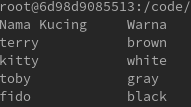
\includegraphics{1.png}
\end{center}

\subsubsection{Praktik 2}
\begin{lstlisting}
public class Array2a {
    public static void main(String[] args) {
        String cats[][]= {{"terry","brown"},
        {"kitty","white"},
        {"toby","gray"},
        {"fido","black"}};
        System.out.println("Nama Kucing\tWarna");
        for (int i=0;i<cats.length;i++) {
            for (int j=0;j<cats[i].length;j++) {
                System.out.print(cats[i][j]);
                System.out.print("\t");
            }
            System.out.println(" ");
        }
    }
}
\end{lstlisting}
Pada praktik 2, adalah mengubah program pada praktik 1, yang semula cara mengeprintnya secara manual, pada praktik 2 dimodifikasi agar mengeprint menggunakan 
perulangan. Karena arraynya mreupakan array dua dimensi, maka digunakan dua perulangan. Yang perulangan pertama berguna untuk menghitung baris, dan perulangan 
kedua untuk menghitung kolom.
\begin{center}
    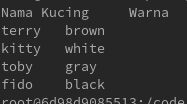
\includegraphics{2.png}
\end{center}

\subsubsection{Praktik 3}
\begin{lstlisting}
import java.util.Scanner;
public class Array2b {
    public static void main(String[] args) {
        String cats[][] = new String[4][2];
        Scanner in = new Scanner(System.in);
        for (int i=0;i<cats.length;i++) {
            for (int j=0;j<cats[i].length;j++) {
                cats[i][j] = in.nextLine();
            }
        }
        System.out.println("Nama Kucing\tWarna");
        for (int i=0;i<cats.length;i++) {
            for (int j=0;j<cats[i].length;j++) {
                System.out.print(cats[i][j]);
                System.out.print("\t");
            }
            System.out.println(" ");
        }
    }
}
\end{lstlisting}
Program tersebut merupakan program dari praktik 2, yang dimodifikasi sehingga mampu menerima input dari user. Perulangan yang digunakan untuk mneginputkan
sama dengan perulangan yang sebelumnya digunakan untuk mengeprint array, sehingga input pertama akan memasukkan nama kucing, dan 
input kedua akan memasukkna warna kucing.
\begin{center}
    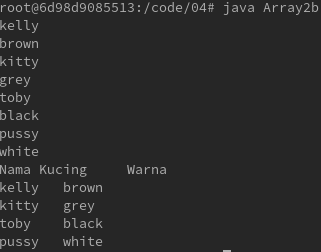
\includegraphics{3.png}
\end{center}

\subsubsection{Praktik 4}
\begin{lstlisting}
import java.util.Scanner;
public class Matrik {
    public static void main(String[] args) {
        Scanner input = new Scanner(System.in);
        int[][] x = {{1, 2, 3}, {4, 5, 6}};
        int[][] y = {{3, 6, 1}, {4, 7, 9}};
        int baris = 2;
        int kolom = 3;
        int[][] z = new int[baris][kolom];
        System.out.println("ini adalah matrix x");
        for (int i = 0; i < baris; i++) {
            for (int j = 0; j < kolom; j++) {
                System.out.print(x[i][j] + " ");
            }
            System.out.println();
        }
        System.out.println("ini adalah matrix y");
        for (int i = 0; i < baris; i++) {
            for (int j = 0; j < kolom; j++) {
                System.out.print(y[i][j] + " ");
            }
            System.out.println();
        }
    }
}
\end{lstlisting}
Pada praktik 4 program memiliki dua array yang berisi matrix. Kemudian kedua matriks tersebut diprint menggunakan perulangan seperti program pada praktik 2.
\begin{center}
    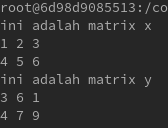
\includegraphics{4.png}
\end{center}

\subsubsection{Praktik 5}
\begin{lstlisting}
import java.util.Scanner;
public class Matrika {
    public static void main(String[] args) {
        Scanner input = new Scanner(System.in);
        int[][] x = {{1, 2, 3}, {4, 5, 6}};
        int[][] y = {{3, 6, 1}, {4, 7, 9}};
        int baris = 2;
        int kolom = 3;
        int[][] z = new int[baris][kolom];
        System.out.println("ini adalah matrix x");
        for (int i = 0; i < baris; i++) {
            for (int j = 0; j < kolom; j++) {
                System.out.print(x[i][j] + " ");
            }
            System.out.println();
        }
        System.out.println("ini adalah matrix y");
        for (int i = 0; i < baris; i++) {
            for (int j = 0; j < kolom; j++) {
                System.out.print(y[i][j] + " ");
            }
            System.out.println();
        }
        System.out.println("hasil dari x-y");
        for (int i = 0; i < baris; i++) {
            for (int j = 0; j < kolom; j++) {
                z[i][j]=x[i][j]-y[i][j];
                System.out.print(z[i][j]+" ");
            }
            System.out.println();
        }
        System.out.println("hasil dari x+y");
        for (int i = 0; i < baris; i++) {
            for (int j = 0; j < kolom; j++) {
                z[i][j]=x[i][j]+y[i][j];
                System.out.print(z[i][j]+" ");
            }
            System.out.println();
        }
    }
}
\end{lstlisting}
Praktik 5 adalah memodifikasi dari praktik 4, sehingga bisa melakukan operasi penambahan dan pengurangan pada matrix yang di masukkan. Pada perulangan 
pertama dan kedua program akan menginputkan matriks pertama dan kedua menginputkan matriks. Perulangan kedua akan mengurangi matriks x dengan matriks y, 
dengan mengurangi baris dengan baris, dan kolom dengan kolom, kemudian mengeprintnya. Kemudian perulangan ketiga akan menambahkan matriks x dengan matriks y, baris dengan baris, kolom dengan kolom, kemudian mengeprintnya.
\begin{center}
    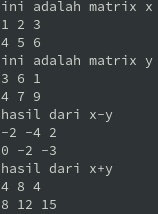
\includegraphics{5.png}
\end{center}

\subsubsection{Praktik 6}
\begin{lstlisting}
public class MatriksTranspose {
    public static void main(String[] args) {
        int[][] matriks =
        {{12,23,32},{34,56,63},{78,89,97}};
        int j,k;
        System.out.println("Matriks Sebelum Transpose");
        for(j=0;j<3;j++){
            for(k=0;k<3;k++){
                System.out.print(matriks[j][k]+" ");
            }
            System.out.println();
        }
        System.out.println("\nMatriks Setelah Transpose");
        for(j=0;j<3;j++){
            for(k=0;k<3;k++){
                System.out.print(matriks[k][j]+" ");
            }
            System.out.println();
        }
    }
}
\end{lstlisting}
Program praktik 6 akan menjalankan operasi transpose terhadap array matriks. Untuk melakukannya digunakan perulangan, yang semula perulangan pertama untuk 
menhitung baris, dan perulangan kedua untuk kolom, dibalik sehingga perulangan pertama untuk menghitung kolom, dan perulangan kedua untuk menghitung baris.
\begin{center}
    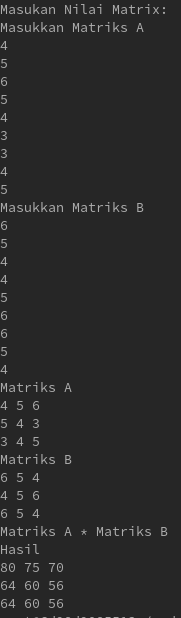
\includegraphics{6.png}
\end{center}

\subsubsection{Praktik 7}
Untuk praktik 7 dibuat program yang akan menginputkan nilai dari matriks 3x3 dan menampilkannya di layar.
\begin{lstlisting}
import java.util.Scanner;
public class Array2Dimensi1 {
    public static void main(String[] args){
        int b=3;int d=3; //matrik 3 baris 3 kolom
        System.out.println("Masukan Nilai Matrix:");
        int[][] matrix1=new int[b][d];
        for(int i=0;i<b;i++){
            for(int j=0;j<d;j++){
                matrix1[i][j]=input();
            }
        }
        for(int i=0;i<b;i++){
            for(int j=0;j<d;j++){
                System.out.print(matrix1[i][j]+" ");
            }
            System.out.println();
        }
    }
    static int input(){
        Scanner a=new Scanner(System.in);
        int b=a.nextInt();
        return b;
    }
}
\end{lstlisting}
Sama dengan program pada praktik 3, disini digunakan perulangan for untuk memasukkan nilai ke dalam matriks. Pengisiannya dengan cara baris demi baris.
\begin{center}
    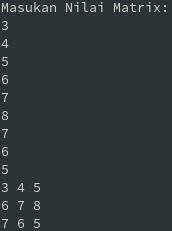
\includegraphics{7.png}
\end{center}

\subsubsection{Praktik 8}
Praktik 8 adalah memodifikasi program dari praktik 7 agar bisa menjalankan operasi perkalian antar matriks.
\begin{lstlisting}
import java.util.Scanner;
public class Array2Dimensi1a {
    public static void main(String[] args){
        int b=3;int d=3; //matrik 3 baris 3 kolom
        System.out.println("Masukan Nilai Matrix:");
        int[][] matrix1=new int[b][d];
        int[][] matrix2=new int[b][d];
        int[][] matrix3=new int[b][d];
        System.out.println("Masukkan Matriks A");
        for(int i=0;i<b;i++){
            for(int j=0;j<d;j++){
                matrix3[i][j] = 0;
                matrix1[i][j]=input();
            }
        }
        System.out.println("Masukkan Matriks B");
        for(int i=0;i<b;i++){
            for(int j=0;j<d;j++){
                matrix2[i][j]=input();
            }
        }
        System.out.println("Matriks A");
        for(int i=0;i<b;i++){
            for(int j=0;j<d;j++){
                System.out.print(matrix1[i][j]+" ");
            }
            System.out.println();
        }
        System.out.println("Matriks B");
        for(int i=0;i<b;i++){
            for(int j=0;j<d;j++){
                System.out.print(matrix2[i][j]+" ");
            }
            System.out.println();
        }
        System.out.println("Matriks A * Matriks B");
        for(int i=0;i<b;i++){
            for(int j=0;j<d;j++){
                matrix3[i][j] = 0;
                for(int k=0;k<d;k++){
                    matrix3[i][j] = matrix1[i][k] * matrix2[k][j] + matrix3[i][j];
                }
            }
        }
        System.out.println("Hasil");
        for(int i=0;i<b;i++){
            for(int j=0;j<d;j++){
                System.out.print(matrix3[i][j]+" ");
            }
            System.out.println();
        }
    }
    static int input(){
        Scanner a=new Scanner(System.in);
        int b=a.nextInt();
        return b;
    }
}
\end{lstlisting}
Pada program tersebut terdapat beberapa perulangan bertingkat. Perulangan bertingkat pertama dan kedua berfungsi untuk memasukkan nilai dari matriks dari user. Perulangan bertingkat ketiga dan keempat berfungsi
untuk menampilkan matriks1 dan matriks 2. Sedangkan perulangan bertingkat ke lima berfungsi untuk memberi nilai 0 pada matriks3, agar nilai tidak null, Lalu akan mengkalikan baris dengan kolom 
lalu akan menambahkannya. Karena rumus perkalian dari matriks seperti berikut:
\begin{center}
    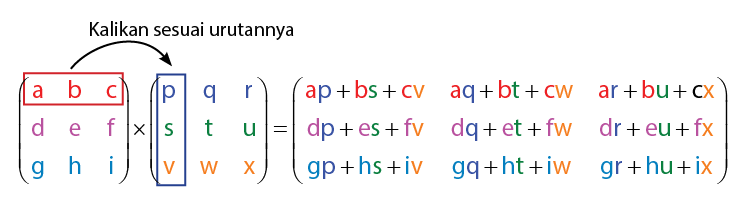
\includegraphics[width=\linewidth]{rumus.png}
\end{center}
Lalu perulangan bertingkat yang terakhir adalah untuk menampilkan matriks3, dimana kita menyimpan hasil operasi perkalian matriks1 dengan matriks 3 tadi. Jadi jika program dijalankan akan 
menghasilkan output seperti berikut:
\begin{center}
    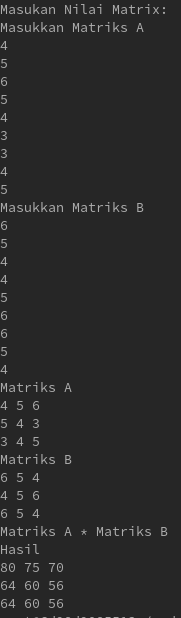
\includegraphics{8.png}
\end{center}

\subsection{Latihan}
\subsubsection{Latihan 1}
Untuk latihan dibuat program untuk menampilkan data nilai mahasiswa.
\begin{lstlisting}
import java.util.Scanner;
public class JavaApplication2 {
    public static void main(String[] args) throws Exception {
        Scanner input = new Scanner(System.in);
        int mhs,jml, banyakTes = 3, nilai[][], ntt[], ntr[];
        float rata[], jumlah[], rtt, rtr;
        System.out.print("Masukkan Jumlah Mahasiswa : ");
        mhs = input.nextInt();
        nilai = new int[mhs][banyakTes];
        jumlah = new float[mhs];
        rata = new float[mhs];
        ntt = new int[banyakTes];
        ntr = new int[banyakTes];
        System.out.println();
        for(int h=0;h<mhs;h++){ //Mahasiswa
            System.out.println("Mahasiswa " + (h+1));
            for(int i=0;i<banyakTes;i++){ //Tes keberapa
                System.out.print("Nilai Tes " + (i+1) + " : ");
                nilai[h][i] = input.nextInt();
                jumlah[h] = jumlah[h] + nilai[h][i];
            }
            rata[h] = jumlah[h]/banyakTes;
            System.out.println();
        }
        for(int i=0;i<banyakTes;i++){
            ntt[i] = nilai[0][i];
            ntr[i] = nilai[0][i];
        }
        rtt = rata[0];
        rtr = rata[0];
        for(int i=0;i<banyakTes;i++){
            for(int j=0;j<mhs;j++){
                if(ntt[i] < nilai[j][i]){
                    ntt[i] = nilai[j][i];
                }
                if(ntr[i] > nilai[j][i]){
                    ntr[i] = nilai[j][i];
                }
            }
        }
        for(int i=0;i<mhs;i++){
            if(rtt < rata[i]){
                rtt = rata[i];
            }
            if(rtr > rata[i]){
                rtr = rata[i];
            }
        }
        System.out.println("---------------------------");
        System.out.println("Daftar Nilai Mahasiswa : ");
        System.out.println("---------------------------");
        System.out.println();
        System.out.println("\t\tTest 1\tTest 2\tTest 3\tRata- rata");
        for(int j=0;j<mhs;j++){
            System.out.print("Mahasiswa " + (j+1));
            for(int k=0;k<banyakTes;k++){
                System.out.print("\t" + nilai[j][k]);
            }
            System.out.print("\t" + rata[j]);
            System.out.println();
        }
        System.out.println();
        System.out.print("Nilai Tertinggi\t");
        for(int j=0;j<banyakTes;j++){//Nilai tertinggi
            System.out.print(ntt[j] + "\t");
        }
        System.out.print(rtt);//Rata-rata tertinggi
        System.out.println();
        System.out.print("Nilai Teredah\t");
        for(int j=0;j<banyakTes;j++){//Nilai terendah
            System.out.print(ntr[j] + "\t");
        }
        System.out.print(rtr);//Rata-rata terendah
        System.out.println();
    }
}
\end{lstlisting}
Dari program di atas terdapat beberapa perulangan. Perulangan pertama berbentuk perulangan bertingkat, perulangan tersebut berfungsi untuk menginputkan banyak
mahasiswa dan menginputkan nilai. kemudian perulangan selanjutnya berguna untuk memberi nilai ke array ntt dan ntr. Perulangan ketiga berguna untuk membandingkan 
nilai pada array nilai. Selanjutnya perulangan keempat erguna untuk mencari rata-rata. Lalu perulangan seterusnya berguna untuk menampilkan variabel array ke layar.
\begin{center}
    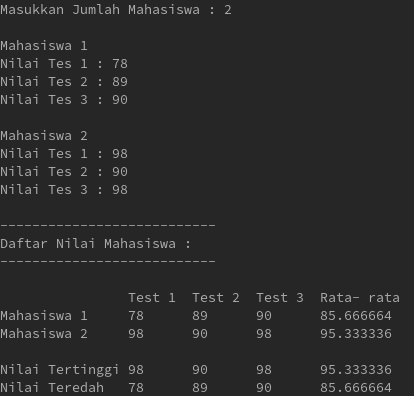
\includegraphics{9.png}
\end{center}

\subsubsection{Latihan 2}
Untuk Latihan kedua adalah memodifikasi latihan pertama supaya program mampu menerima input nim, nama, dan jurusan. 
\begin{lstlisting}
import java.util.Scanner;
public class JavaApplication2a {
    public static void main(String[] args) throws Exception {
        Scanner input = new Scanner(System.in);
        int mhs,jml, banyakTes = 3, nilai[][], ntt[], ntr[];
        float rata[], jumlah[], rtt, rtr;
        System.out.print("Masukkan Jumlah Mahasiswa : ");
        mhs = input.nextInt();
        nilai = new int[mhs][banyakTes];
        jumlah = new float[mhs];
        rata = new float[mhs];
        ntt = new int[banyakTes];
        ntr = new int[banyakTes];
        String[] nama = new String[mhs];
        String[] nim = new String[mhs];
        String[] jur = new String[mhs];
        System.out.println();
        for(int h=0;h<mhs;h++){ //Mahasiswa
            System.out.println("Mahasiswa " + (h+1));
            input.nextLine();
            nama[h] = input.nextLine();
            nim[h] = input.nextLine();
            jur[h] = input.nextLine();
            for(int i=0;i<banyakTes;i++){ //Tes keberapa
                System.out.print("Nilai Tes " + (i+1) + " : ");
                nilai[h][i] = input.nextInt();
                jumlah[h] = jumlah[h] + nilai[h][i];
            }
            rata[h] = jumlah[h]/banyakTes;
            System.out.println();
        }
        for(int i=0;i<banyakTes;i++){
            ntt[i] = nilai[0][i];
            ntr[i] = nilai[0][i];
        }
        rtt = rata[0];
        rtr = rata[0];
        for(int i=0;i<banyakTes;i++){
            for(int j=0;j<mhs;j++){
                if(ntt[i] < nilai[j][i]){
                    ntt[i] = nilai[j][i];
                }
                if(ntr[i] > nilai[j][i]){
                    ntr[i] = nilai[j][i];
                }
            }
        }
        for(int i=0;i<mhs;i++){
            if(rtt < rata[i]){
                rtt = rata[i];
            }
            if(rtr > rata[i]){
                rtr = rata[i];
            }
        }
        System.out.println("---------------------------");
        System.out.println("Daftar Nilai Mahasiswa : ");
        System.out.println("---------------------------");
        System.out.println();
        System.out.println("\t\t\tTest 1\tTest 2\tTest 3\tRata- rata");
        for(int j=0;j<mhs;j++){
            System.out.print(nama[j]+"\t"+nim[j]+"\t"+jur[j]);
            for(int k=0;k<banyakTes;k++){
                System.out.print("\t" + nilai[j][k]);
            }
            System.out.print("\t" + rata[j]);
            System.out.println();
        }
        System.out.println();
        System.out.print("Nilai Tertinggi\t");
        for(int j=0;j<banyakTes;j++){//Nilai tertinggi
            System.out.print(ntt[j] + "\t");
        }
        System.out.print(rtt);//Rata-rata tertinggi
        System.out.println();
        System.out.print("Nilai Teredah\t");
        for(int j=0;j<banyakTes;j++){//Nilai terendah
            System.out.print(ntr[j] + "\t");
        }
        System.out.print(rtr);//Rata-rata terendah
        System.out.println();
    }
}
\end{lstlisting}
Pada program tersebut ditambahkan variabel array 1 dimensi, yaitu nim, nama, dan jur. Untuk pengisiannya digunakan perulangan for yang merupakan perulangan pertama.
lalu untuk menampilkannya juga digunakan perulangan for.

\newpage

\section{Kesimpulan}
Setelah praktik mahasiswa mampu menjelaskan konsep array 2 dimensi, merencanakan struktur data dalam bentuk array 2 dimensi, mengaplikasikan array 2 dimensi.

\end{document}
